%%%%%%%%%%%%%%%%%%%%%%%%%%%%%%%%%%%%%%%%%%%%%%%%%%%%%%%%%%%%%%%%%%%%%%%%%%%%%%%%
%2345678901234567890123456789012345678901234567890123456789012345678901234567890
%        1         2         3         4         5         6         7         8

\documentclass[letterpaper, 10 pt, conference]{ieeeconf}  % Comment this line out if you need a4paper
\usepackage{verbatim}
%\documentclass[a4paper, 10pt, conference]{ieeeconf}      % Use this line for a4 paper

\IEEEoverridecommandlockouts                              % This command is only needed if 
                                                          % you want to use the \thanks command

\overrideIEEEmargins                                      % Needed to meet printer requirements.

% See the \addtolength command later in the file to balance the column lengths
% on the last page of the document

% The following packages can be found on http:\\www.ctan.org
%\usepackage{graphics} % for pdf, bitmapped graphics files
\usepackage[pdftex]{graphicx}
\graphicspath{{./img/}}
\DeclareGraphicsExtensions{.pdf,.png,.jpg}


%\usepackage{epsfig} % for postscript graphics files
%\usepackage{mathptmx} % assumes new font selection scheme installed
%\usepackage{times} % assumes new font selection scheme installed
%\usepackage{amsmath} % assumes amsmath package installed
%\usepackage{amssymb}  % assumes amsmath package installed

\usepackage[usenames,dvipsnames,svgnames,table]{xcolor}


\newcommand\jp[1]{{\color{red}}{\color{red}}{\footnotesize \color{red}[#1 - \textbf{Jordi}]}} %jp for Jordi
\newcommand\cmf[1]{{\footnotesize \color{red}[#1 - \textbf{Cl\'ement}]}} %CMF for Clément
\newcommand\vv[1]{{\color{red}}{\color{red}}{\footnotesize \color{red}[#1 - \textbf{Vicky}]}} %vv for vicky
\newcommand\ih[1]{{\color{red}}{\color{red}}{\footnotesize \color{red}[#1 - \textbf{Ivan}]}} %ih for ivan
\newcommand\ms[1]{{\color{red}}{\color{red}}{\footnotesize \color{red}[#1 - \textbf{Marti}]}} %ms for Marti

\title{\LARGE \bf
%Learning Abstractions from Human Teachers(or some cooler title)*\\
Skill refinement through cerebellar learning and human haptic feedback:
an iCub learning to paint experiment*
}


\author{Jodir-Ysard Puigb\`o$^{1}$, Cl\'{e}ment Moulin-Frier$^{1}$, Vasiliki Voulutsi$^{1}$,\\ Mart\'i Sanchez-Fibla$^{1}$, Ivan Herreros$^{1}$ and Paul FMJ. Verschure$^{1,2}$, % <-this % stops a space
\thanks{*This work was partially supported by WYSIWYD (add FP7 grant). CMF: check with Marti and Paul if we mention SocSMCs or CDAC as well. }% <-this % stops a space
\thanks{$^{1}$Synthetic Perceptual Emotive and Cognitive Systems Laboratory, Department of Comunication and Technology, Universitat Pompeu Fabra
        {\tt\small albert.author@papercept.net}}%
\thanks{$^{2}$ICREA (Check how this finishes)
        }%
}


\begin{document}



\maketitle
\thispagestyle{empty}
\pagestyle{empty}


%%%%%%%%%%%%%%%%%%%%%%%%%%%%%%%%%%%%%%%%%%%%%%%%%%%%%%%%%%%%%%%%%%%%%%%%%%%%%%%%
\begin{abstract}
 % Shouldn't ocupy more thant one paragraph (around 100-200 words)
This article presents a model of the control of hand movements learned from human imprecise feedback. 
The setup consists in an iCub humanoid robot able to paint with its finger tip on an interactive display. It learns to avoid an abstract boundary, which is drawn on the table and that the robot can perceive. Before learning, the robot does not know that it has to paint only inside the boundary. This is instead learned from human feedback provided whenever the robot’s finger tip goes outside of the shape. We use a neurocomputational model of the cerebellum, which learns to anticipate the human feedback from the perception of the, previously meaningless shape boundaries. 

We show how this biologically-inspired adaptive mechanism, which is plausible in term of human infant development, allows the learning of a precise painting behavior, using the perception of the shape boundaries as a predictive signal of negative feedback. This mechanism can be generalized to any kind of task where negative feedback can be predicted by sensory cues.


... in the direction of a two-phase model...


\end{abstract}



%%%%%%%%%%%%%%%%%%%%%%%%%%%%%%%%%%%%%%%%%%%%%%%%%%%%%%%%%%%%%%%%%%%%%%%%%%%%%%%%
\section{INTRODUCTION}
%This should not be more than finishing this page...

\textbf{Clement starts:} Humanoids robots are of special interest when it comes to socially interact with non-expert human users since their anthropomorphic shapes foster natural interactions as they can be observed between human conspecifics. However, how such natural interactions can be used for social learning, i.e. for the acquisition of relevant skills by knowledge transfer from the user to the robot, is still considered as a difficult problem despite the number of contributions in the field. (CMF: any refs on this, perhaps Vicky?)

A particular problem is the learning of task constraints from user feedback. In this case the user does not provide information about the way of performing a particular task (this is the domain of learning by demonstration which is outside the scope of this paper), but only about whether the current behavior of the robot is considered as appropriate or not by the user to actually perform the task. Therefore, the problem faced by the robot is how to interpret the user feedback to adapt its own behavior in order to maximize the amount of rewarding stimuli and minimize the amount of aversive ones.

This problem of social learning from human feedback has often been considered as a reinforcement learning (RL) problem. In that context, a number of efficient algorithm from the RL literature can be applied to optimize the robot action policy in the sake of maximizing the cumulative future reward, which is here directly related to the user feedback. However, the fact that human reinforcement is often noisy can be a challenging problem.

In this paper, we rather address the problem by adopting a biologically-grounded approach based on our previous work on neurocomputational models of reactive and adaptive control. We take inspiration from the classical conditioning paradigm (Pavlov et al., 1927). It has been observed that animals learn to anticipate aversive stimuli when it is presented shortly after consistent contextual information. A typical example is an animal learning to anticipate eye-blinking to avoid an air puff which is consistently presented after a tone (Gormezano, 1987). This learning process has been precisely targeted inside the cerebellum (Christian et al., 2003; Yeo et al.1998) and we have recently proposed a neurocomputational model of this brain structure (Herreros et al., 2013a) to anticipate the aversive stimuli from the perception of contextual clues. 

\textbf{Clement ends}

\textbf{Marti starts:}
We address a robot painting training scenario via cerebellar learning with human haptic feedback. Our contribution is twofold: firstly we use a neurophysiological plausible model of the  cerebellum  \cite{herreros2013nucleo} which is used to exploit the anticipation of the, so called Unconditioned Stimulus (US), which in our painting scenario is triggered when surpassing the border of the area that has to be painted (filled). Secondly we use unspecific and imprecise human tactile feedback (delivered to the forearm of the iCub) to drive learning, so that the signalling of the US is driven by this haptic feedback, with no previous notion of border.

Robotics and neuroscience are fields in fruitful collaboration \cite{floreano2014robotics}, and we exactly place our contributions in this intersection by proposing a complete system implementing the minimal components of a developmental scenario in which the iCub robot learns a skill through human feedback by acquiring the adaptive motor responses using a biologically valid model of the cerebellum.

In our view, behaviour is organised in a layered structure building bottom up from a reactive component and adding, through learning, an adaptive contribution
as in the Distributed Adaptive Control architecture (DAC) \cite{verschure2003environmentally} (contextual aspects of the task are out of the scope of the paper). In our task we learn from a reactive controller, exploiting the anticipation provided by cerebellar learning, producing an additional adaptive component that refines and makes the execution of the task more precise. 

Neurophysiological models of the cerebellum are becoming popular in robotics, although to our knowledge, they have not been used in a complete developmental scenario including human feedback. In \cite{hofstoetter2002cerebellum} a mobile robot learns to avoid collisions. The same cerebellar model has been applied for anticipating the turning action of a robot in a rapid navigation task  \cite{herreros2013speed} (which addresses generalization properties of the cerebellar learning). Examples of postural and position control tasks are described in \cite{pinzon2015realistic}, in which spiking models of the cerebellum are used. \cite{barron2013cerebellum} uses cerebellar based adaptation to refine the precision of an arm control task when exploring a surface of uncertain depth. In our case we enhance the precision of the arm movement with the goal of painting a predefined area without surpassing the borders.   

On the other hand, we think that training by human feedback (as in \cite{knox2013training}) can benefit from our minimal real-world biologically valid implementation.


% Marti: for the Discussion 
The cerebellar model is a supervised learning system that in our case is driven by an unspecific error from human feedback, unspecific in the sense that it only signals the aversive state but it does not contain information of how to correct it. The trick is that learning is anticipating the triggering of the reactive behaviour in advance which in itself contains information on the movement to make.
In the future we will consider of making the human feedback more specific, by for example being able to translate a tactile pattern, while holding the forearm of the iCub, into a correcting direction. We could consider as well using the force feedback sensing of the iCub for this purpose.

\textbf{Marti ends}


% **********************************************************************

\textbf{Jordi starts}

Robot control is an open problem that grows with the complexity of the tasks. Specially, contextual information is usually difficult to handle. While classical control algorithms fail if not all the possible conditions are foreseen, common machine learning approaches tend to fail due to overfitting to in-lab environments or lack of generalization for never experienced situations. 
Trying to solve this problem, back on the ¿nineties?, severeal attempts to approach the problem in a different way were proposed, including evolutionary algorithms, more adaptive, plastic and biologically grounded controllers (cite here rodney brooks, gerald edelman and look for some other important references). This approaches, specially those based on evolution or error detection, need the robot to fail to then acquire better mechanisms to interact with their environment. While these techniques are feasible in simulations or simple or cheap robots, trying to apply evolution of algorithms to more complex machinery lead to exponential increases in experimental time and resource costs. This, applied to extreme cases as humanoid robots with several tens of degrees of freedom and even more sensors, make the application of this kind of tasks unfeasible. 

In the case of humanoid robots, but not limited to it, a common approach is to emulate the development of cognitive functions in children or animal offspring. The acquisition of meaning from the environment is one of the main goals associated to the field of developmental robotics. In this specific case, we are using an iCub robot [add reference] and we look at the way knowledge is transmitted from adults to children. 

One of the ways neuroscience attacks the problem of knowledge acquisition is through conditioning. It has been observed that animals learn to anticipate both, reward and aversive stimuli after exposure to the stimuli and some consistent contextual information. An example would be (pavlov and dog? the eyeblink?). In the case of aversive stimuli, the process by which conditioning happens has been precisely targeted inside the cerebellum, in what is called classical conditioning. We are using this approach to let the robot learn to anticipate an aversive stimulus coming from the human, as could be excessive pressure on tactile skin, using contextual data from other sensors, therefore leading to the implicit association of a previously meaningless pattern to a specific action. 

...ADD SOMETHING ELSE HERE?...


This article is organized as follows: section \ref{sec:neuro} provides details about the controller and its neurological substrate. Next, section \ref{sec:setup} describes the experimental setup to describe the results in \ref{sec:results}. Finally, section \ref{sec:conclusions} promotes discussion and introduces ongoing and future work. 



\section{Neuro-controller}
\label{sec:neuro}
Homeostasis + Cerebellum in roboticist words

Our model consists of an adaptive controller on top of a reactive one. With this design, the reactive controller serves the goal of keeping a series of needs in a comfort zone (CZ) every time its boundary is crossed, through automatic, predefined action (or reflex). On top of it, the adaptive controller has the role of anticipating when the boundary of the CZ is about to be crossed. With this objective, the adaptive controller generates or modifies behavior, learning from contextual sensory cues. It is important to note that this contextual cues have been present all the time, although they had no relevance. After learning, those cues that are relevant for avoiding stimuli are identified and used with such a goal. 

\subsection{Reactive Controller: Homeostasis}
\cmf{I would rather move all the biological stuff either in the intro or a dedicated section, focusing here on the model}
When an animal is in presence of excessive temperature, hunger, pain, etc. its body tends to generate behaviors that compensate for these excesses through self-regulation. Homeostasis is the biological mechanism by which self-regulation is maintained and allows animals to adapt to ever changing environment and body conditions. Homeostasis can be globally understood as the set of needs and drives that govern an animal's behavior. 
We have designed a, purely reactive, homeostatic controller that defines a series of needs and links them to predefined actions. Our model generally defines a need or drive as a CZ in some sensory dimension. The boundaries of this CZ are defined as thresholds on this sensory dimension. The reactive controller generates reflexes that react to surpassing the boundaries of this CZ.  Surpassing the threshold triggers an action that, ideally, brings the measurement back to the CZ. Must be noted that, in the lowest implementation of the controller, the reflexes are not precise actions, but overreactions that ensure that the measure is back to safety. An example of a homeostatic drive could be the sense of contact on the skin of a robot, or its force/torque sensors . The reactive controller receives a signal when these sensors go out of the CZ and generates a general movement action on the opposite direction associated to the sensor. 
Entering higher cognitive functions, homeostasis can then be generally understood as any other abstract need or drive of the robot. These needs can then also be associated to higher level actions. This means that we could define a reflex that associates excessive pressure with reverting the previous action, as a more global need to satisfy human intentions. BLABLALBA

The model that we used is based on Vicky \& Stephane reference.

To types of drives: gradient based or decay based

\subsection{Adaptive Controller: Cerebellum}

On top of the reactive controller we use a model of the cerebellum, which acts as an adaptive controller. The cerebellum has been related to sensory-motor prediction and optimization for a long time. The most studied paradigm for the study of the cerebellum is known as Classical Conditioning. In Classical Conditioning, an aversive unconditioned stimulus (US), like an air-puff on the eye, is preceded by a neutral conditioning stimulus that could be a tone. The first presentations of the US-CS pair trigger an automatic unconditioned response that tries to cancel the US, but after a few trials, the circuitry in the cerebellum has learned to anticipate the US. Then, the CS will be the stimulus producing a conditioned response (CR) that will avoid completely or partially the US.

For this paradigm we use the model of the cerebellum \cite{herreros2013nucleo}. This model considers an input (the CS) expanded in the temporal dimension which is used by an adaptive filter that predicts the US. We add an external layer that transforms this prediction into a motor response (the CR). We model the US-UR loop using the homeostatic model presented in the previous section. For more details on the implementation of the adaptive controller we direct the reader to ref[Herreros and Verschure 2012]. 

\subsection{Cognitive architecture}

Bla

\begin{figure}[!t]
\centering
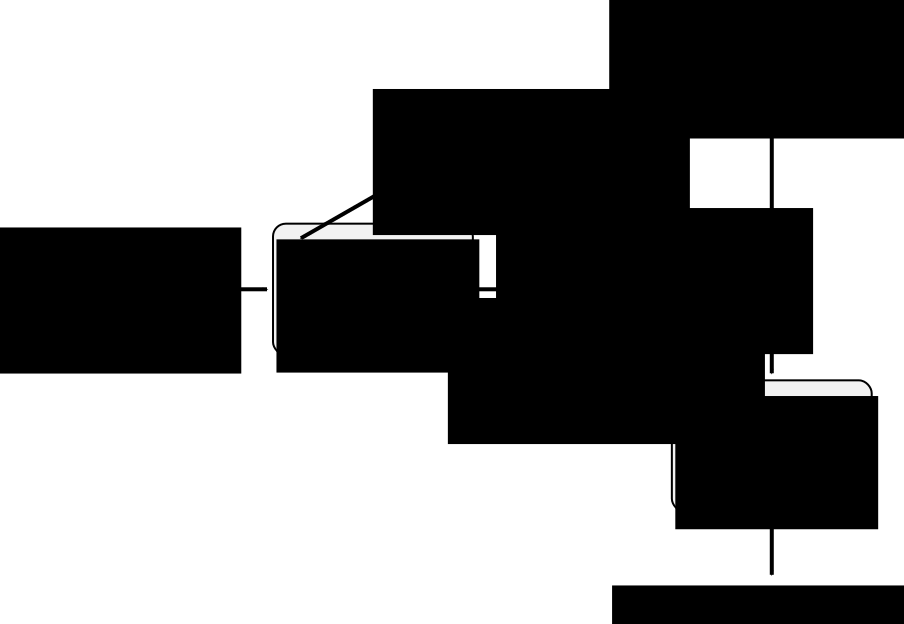
\includegraphics[width=2.5in]{architecture}
\caption{.}
\label{fig:architecture}
\end{figure}

%\subsection{Tying Everything Together}
%In this article we present the combined model of using self-regulation or homeostasis as the generator of the signal that must be anticipated by the cerebellum. In this combination, we chose to use high level needs so that we can generalize 

\section{Educating Robots: Experimental Setup}
\label{sec:setup}
IROS summary + This setup

\section{Results}
\label{sec:results}
Compare both

\section{CONCLUSIONS}
\label{sec:conclusions}

...

It is clear that this system will fail to anticipate when contextual cues are noisy or imprecise. For this reason, we propose the use a two phase model of learning [reference] that, independently from the prediction phase, uses the US [CHECK THAT US HAS BEEN DEFINED BEFORE] to learn to effectively represent significant stimuli (good or bad). This perceptual phase is grounded on the observed increase in plasticity in the sensory cortex in presence aversive or rewarding stimuli. This model should then be able to learn the relevant perceptual blocks that allow a consistent and robust anticipation of reward or punishment. 

...

\addtolength{\textheight}{-12cm}   % This command serves to balance the column lengths
                                  % on the last page of the document manually. It shortens
                                  % the textheight of the last page by a suitable amount.
                                  % This command does not take effect until the next page
                                  % so it should come on the page before the last. Make
                                  % sure that you do not shorten the textheight too much.

%%%%%%%%%%%%%%%%%%%%%%%%%%%%%%%%%%%%%%%%%%%%%%%%%%%%%%%%%%%%%%%%%%%%%%%%%%%%%%%%
\begin{comment}
\section{EUCOG abstract}
We present a model of the control of hand movements learned from human feedback. The setup consists in an iCub humanoid robot able to paint with its finger tip on an interactive display, the Reactable. It learns how to paint inside a closed shape, e.g. a circle, which is drawn on the table and from which the robot can perceive the boundaries. Before learning, the robot does not know that it has to paint only inside the boundaries. This is instead learned from negative human feedback provided whenever the robot’s finger tip goes outside of the shape, using a neurocomputational model of the cerebellum learning how to anticipate the negative feedback from the perception of the shape boundaries. 

Our model consists in a reactive and an adaptive controllers. The reactive controller defines two needs of the robot. The first one drives the robot to move the virtual pen on the table in random directions, without taking into account the perception of the shape boundaries. The second need drives the robot to move the pen in the opposite direction whenever it perceives a negative human feedback. We show that this simple reactive controller, when acting in isolation, allows to roughly paint inside the shape although it often crosses the shape boundaries as an untrained young infant would do.

On top of this purely reactive system, an adaptive controller tries to make sense of the human feedback to optimize behavior, i.e to minimize the amount of negative feedback it will receive -- and consequently to paint with more precision. The adaptive controller aims at learning how to perform anticipatory actions to avoid the human negative feedback. It is based on a neurocomputational model of the cerebellum which functionally acts as a function approximator and learns to predict the negative feedback from the perception of the shape boundaries relatively to the position of the finger tip. Because the human feedback is correlated with the distance between the finger tip and the closest shape edge, the adaptive controller learns to perform the compensatory action, i.e. the moving of the finger tip in the opposite direction, whenever the latter becomes too close from a shape boundary. 

We show how this biologically-inspired adaptive mechanism, which is plausible in term of human infant development, allows the learning of a precise painting behavior, using the perception of the shape boundaries as a predictive signal of negative feedback. This mechanism can be generalized to any kind of task where negative feedback can be predicted by sensory cues.

\end{comment}

%%%%%%%%%%%%%%%%%%%%%%%%%%%%%%%%%%%%%%%%%%%%%%%%%%%%%%%%%%%%%%%%%%%%%%%%%%%%%%%%



%%%%%%%%%%%%%%%%%%%%%%%%%%%%%%%%%%%%%%%%%%%%%%%%%%%%%%%%%%%%%%%%%%%%%%%%%%%%%%%%
\section*{APPENDIX}

Appendixes should appear before the acknowledgment.

\section*{ACKNOWLEDGMENT}

The preferred spelling of the word ÒacknowledgmentÓ in America is without an ÒeÓ after the ÒgÓ. Avoid the stilted expression, ÒOne of us (R. B. G.) thanks . . .Ó  Instead, try ÒR. B. G. thanksÓ. Put sponsor acknowledgments in the unnumbered footnote on the first page.



%%%%%%%%%%%%%%%%%%%%%%%%%%%%%%%%%%%%%%%%%%%%%%%%%%%%%%%%%%%%%%%%%%%%%%%%%%%%%%%%

\bibliographystyle{IEEEtran}
\bibliography{humanoids}





\end{document}